\section{Задача 1.38}
\subsection{Задание:}
Как изменится определитель если в нём:\\
а) к каждой строке, кроме последней, прибавить последнюю строку;\\
б) из каждой строки, кроме последней, вычесть все последующие строки;\\
в) из каждой строки, кроме последней, вычесть последующую строку, а из последней вычесть бывшую первоначально первой;\\
г) повернуть его матрицу на $ 90 $ градусов вокруг центра по часовой стрелке;\\
д) первый столбец поставить на последнее место, сохранив порядок следования остальных столбцов.\\
\subsection{К каждой строке, кроме последней, прибавить последнюю строку:}
По свойству определителя если к любой строке определителя прибавить другую строку определителя, он не изменится.
Значит и в результате данного преобразования определитель не изменится.
\\[1em]
Проверим в компьютерной среде Wolfram Mathematica:
\\
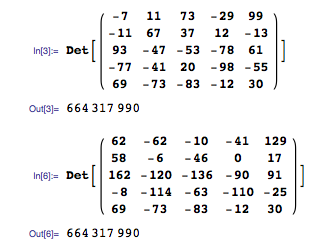
\includegraphics[scale=0.6]{task/1_38/screen1.png}
\subsection{Из каждой строки, кроме последней, вычесть все последующие строки:}
По свойству определителя если к любой строке определителя прибавить линейную комбинацию других строк определителя, он не изменится.
Значит и в результате данного преобразования определитель не изменится.
\\[1em]
Проверим в компьютерной среде Wolfram Mathematica:
\\
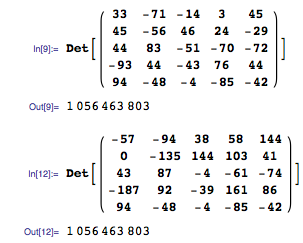
\includegraphics[scale=0.6]{task/1_38/screen2.png}
\subsection{Из каждой строки, кроме последней, вычесть последующую строку, а из последней вычесть бывшую первоначально первой}
Пусть есть матрица $ A $ над которой мы будем производить такую операцию.
Эта операция равнозначна умножению слева матрицы $ A $ на матрицу
$
	B =
	\begin{pmatrix}
		1      & -1     & 0      & \cdots & 0      & 0      \\
		0      & 1      & -1     & \cdots & 0      & 0      \\
		\vdots & \vdots & \vdots & \ddots & \vdots & \vdots \\
		0      & 0      & 0      & \cdots & 1      & -1     \\
		-1     & 0      & 0      & \cdots & 0      & 1      \\
	\end{pmatrix}
$. По свойству определителя $ |BA| = |B| \cdot |A| $. Найдём $ |B| $ разложив его по последней строке:
\\[1em]
$
	B \in M(n)
	\\[1em]
	|B| = (-1)^{n+1} \cdot
	\begin{vmatrix}
		-1     & 0      & \cdots & 0      & 0      \\
		1      & -1     & \cdots & 0      & 0      \\
		\vdots & \vdots & \ddots & \vdots & \vdots \\
		0      & 0      & \cdots & 1      & -1     \\
	\end{vmatrix}
	+
	\begin{vmatrix}
		1      & -1     & 0      & \cdots & 0      \\
		0      & 1      & -1     & \cdots & 0      \\
		\vdots & \vdots & \vdots & \ddots & \vdots \\
		0      & 0      & 0      & \cdots & -1     \\
		0      & 0      & 0      & \cdots & 1      \\
	\end{vmatrix}
	=
	\\[1em]
	=
	(-1)^{n+1} \cdot (-1)^n + 1 = -1 + 1 = 0
$
\\[1em]
Тогда $ |BA| = 0 \cdot |A| = 0 $, в результате такого преобразования определеитель станет равен нулю.
\\[1em]
Проверим в компьютерной среде Wolfram Mathematica:
\\
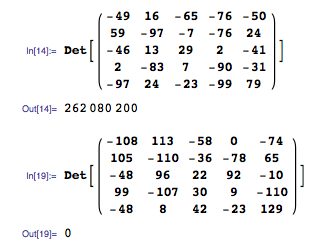
\includegraphics[scale=0.6]{task/1_38/screen3.png}
\subsection{Повернуть его матрицу на $ 90 $ градусов вокруг центра по часовой стрелке}
Чтобы повернуть матрицу на $ 90 $ градусов транспонируем её, а потом умножим справа на матрицу
\\[1em]
$
	B =
	\begin{pmatrix}
		0 & \cdots & 0 & 1 \\
		0 & \cdots & 1 & 0 \\
		\vdots & \ddots & \vdots & \vdots \\
		1 & \cdots & 0 & 0 \\
	\end{pmatrix}
\\
	|B| = (-1)^{\left[\frac{n}{2}\right]}
$ значит изменённый определитель $ |A'| = (-1)^{\left[\frac{n}{2}\right]} \cdot |A| $
\\[1em]
Проверим в компьютерной среде Wolfram Mathematica:
\\
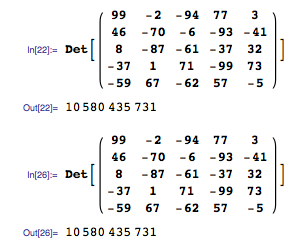
\includegraphics[scale=0.6]{task/1_38/screen4.png}
\subsection{Первый столбец поставить на последнее место, сохранив порядок следования остальных столбцов}
Для этого последовательно будем менять $ i $-ый и $ i+1 $-ый столбцы начиная с $ i = 1 $ до $ n - 1 $.
При каждой замене знак определителя будет меняться на противоположный, всего замен $ n - 1 $, значит $ |A'| = (-1)^{n-1} \cdot |A| $.
\\[1em]
Проверим в компьютерной среде Wolfram Mathematica:
\\
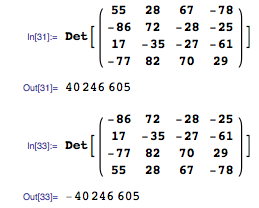
\includegraphics[scale=0.6]{task/1_38/screen5.png}
